\submittedby{Satyajit}

Topologies on $\R$: $\T_f$ (finite complement), $\T_c$ (countable complement), $\T_{\mathrm{std}}$
(basis $(a,b)$), $\T_K$ (basis $(a,b)$ and $(a,b)\setminus K$, $K=\{1,\tfrac12,\tfrac13,\dots\}$),
$\T_\ell$ (basis $[a,b)$), $\T_u$ (basis $(a,b]$), $\T_{\mathrm{left}}$ (basis $(-\infty,b)$),
$\T_{\mathrm{right}}$ (basis $(a,\infty)$).

Here $\T_f=\{\emptyset\}\cup\{U:\R\setminus U\text{ finite}\}$ and
$\T_c=\{\emptyset\}\cup\{U:\R\setminus U\text{ countable}\}$. Also
$\T_{\mathrm{left}}=\{\emptyset,\R\}\cup\{(-\infty,b)\}$ (a union of left rays is a left ray or
$\R$), and similarly $\T_{\mathrm{right}}=\{\emptyset,\R\}\cup\{(a,\infty)\}$.

\textbf{Convention.} $\T\subseteq\T'$ means $\T'$ is \emph{finer}. To show a set is not open in
a topology generated by a basis, show that some point of it lies in no basis element contained
in the set.

\paragraph{Part 1: Inclusions.}

\textbf{1. $\T_f\subsetneq\T_c$.} A finite set is countable, so every nonempty $\T_f$-open set
is in $\T_c$. Strict: $\R\setminus\Q\in\T_c$ (complement $\Q$ countable) but $\notin\T_f$ ($\Q$
infinite).

\textbf{2. $\T_f\subsetneq\T_{\mathrm{std}}$.} If $U=\R\setminus\{x_1<\dots<x_k\}$, then
$U=(-\infty,x_1)\cup(x_1,x_2)\cup\dots\cup(x_k,\infty)$, a union of open intervals (a ray is a
union of bounded intervals, e.g.\ $(-\infty,x_1)=\bigcup_n(x_1-n,x_1)$). Strict:
$(0,1)\in\T_{\mathrm{std}}$ is nonempty with infinite complement, so $\notin\T_f$.

\textbf{3. $\T_{\mathrm{left}},\T_{\mathrm{right}}\subsetneq\T_{\mathrm{std}}$.}
$(-\infty,b)=\bigcup_n(b-n,b)$ and $(a,\infty)=\bigcup_n(a,a+n)$ are standard-open. Strict:
$(0,1)$ is neither $\emptyset$, $\R$, a left ray, nor a right ray, so it is open in neither ray
topology.

\textbf{4. $\T_{\mathrm{std}}\subsetneq\T_K$.} Every $(a,b)$ is a basis element of $\T_K$.
Strict: $(-1,1)\setminus K\in\T_K$ contains $0$, but no interval $(-\delta,\delta)$ lies in it
(it contains $1/n$ for large $n$), so it is not standard-open.

\textbf{5. $\T_{\mathrm{std}}\subsetneq\T_\ell$ and $\T_{\mathrm{std}}\subsetneq\T_u$.}
\[ (a,b)=\bigcup_{x\in(a,b)}[x,b)=\bigcup_{x\in(a,b)}(a,x]. \]
Strict: $[0,1)\in\T_\ell$ is not standard-open (no interval around $0$ fits inside), and
$(0,1]\in\T_u$ is not standard-open (no interval around $1$ fits inside).

\textbf{6. $\T_K\subsetneq\T_u$.} Every $(a,b)$ is standard-open, hence $\T_u$-open. Take
$x\in(a,b)\setminus K$; we find a basis set $(c,x]$ with $x\in(c,x]\subseteq(a,b)\setminus K$:
\begin{itemize}[nosep]
  \item if $x\le0$: take $c=a<x$; then $(a,x]\subseteq(a,b)$ contains no positive numbers,
        hence no point of $K$;
  \item if $x>0$: let $k=\max\{1/n:1/n<x\}=1/n_0$ with $n_0$ the least integer $>1/x$, and
        $c=\max(a,k)<x$. Every element of $K$ that is $<x$ is $\le k\le c$, and $x\notin K$, so
        $(c,x]\cap K=\emptyset$ and $(c,x]\subseteq(a,b)\setminus K$.
\end{itemize}
Thus $(a,b)\setminus K$ is a union of members of $\B_4$, i.e.\ $\T_u$-open. Strict:
$(0,1]\in\T_u$ but $\notin\T_K$: a $\T_K$ basis element containing $1$ cannot be of the form
$(a,b)\setminus K$ (as $1\in K$), so it is an interval $(a,b)$ with $b>1$, which is not
contained in $(0,1]$.

\textbf{7. Transitive consequences.}
$\T_f\subsetneq\T_{\mathrm{std}}\subsetneq\T_K,\T_\ell,\T_u$, so $\T_f$ is strictly coarser than
all of $\T_K,\T_\ell,\T_u$; likewise $\T_{\mathrm{left}},\T_{\mathrm{right}}$ are strictly
coarser than $\T_K,\T_\ell,\T_u$, and $\T_{\mathrm{std}}\subsetneq\T_u$.

\paragraph{Part 2: Incomparable pairs (with witnesses).}
\begin{itemize}
  \item \textbf{$\T_K$ and $\T_\ell$.} $(-1,1)\setminus K\in\T_K\setminus\T_\ell$: every
        $[0,\varepsilon)$ contains some $1/n$. $[0,1)\in\T_\ell\setminus\T_K$: every
        $\T_K$-basis element containing $0$ contains negative numbers.
  \item \textbf{$\T_\ell$ and $\T_u$.} $[0,1)\in\T_\ell\setminus\T_u$ (every $(c,0]$ contains
        negatives); $(0,1]\in\T_u\setminus\T_\ell$ (every $[1,\varepsilon)$ contains numbers
        $>1$).
  \item \textbf{$\T_{\mathrm{left}}$ and $\T_{\mathrm{right}}$.}
        $(-\infty,0)\in\T_{\mathrm{left}}\setminus\T_{\mathrm{right}}$ and
        $(0,\infty)\in\T_{\mathrm{right}}\setminus\T_{\mathrm{left}}$.
  \item \textbf{$\T_f$ and each ray topology.} $(-\infty,0)\in\T_{\mathrm{left}}$ has infinite
        complement, so $\notin\T_f$; and $\R\setminus\{0\}\in\T_f$ is not a left ray nor $\R$,
        so $\notin\T_{\mathrm{left}}$. The same witnesses (with $(0,\infty)$) work for
        $\T_{\mathrm{right}}$.
  \item \textbf{$\T_c$ and each of $\T_{\mathrm{std}},\T_K,\T_\ell,\T_u,\T_{\mathrm{left}},
        \T_{\mathrm{right}}$.}
        \begin{itemize}[nosep]
          \item $\R\setminus\Q\in\T_c$ is not open in any of the six: every nonempty open set
                of each contains a nonempty interval minus at most $K$ (or a half-open interval
                or a ray), hence contains rational numbers.
          \item Conversely $(0,1)\in\T_{\mathrm{std}}\subseteq\T_K,\T_\ell,\T_u$ is open in them
                but $\notin\T_c$ (its complement is uncountable); and
                $(-\infty,0)\in\T_{\mathrm{left}}$, $(0,\infty)\in\T_{\mathrm{right}}$ are not in
                $\T_c$ for the same reason.
        \end{itemize}
\end{itemize}

\paragraph{Comparison table.}
Entry in row $R$, column $C$: $\subsetneq$ means $\T_R$ is strictly coarser than $\T_C$;
$\supsetneq$ strictly finer; $\parallel$ incomparable.

\begin{center}
\small
\renewcommand{\arraystretch}{1.3}
\begin{tabular}{c|cccccccc}
 & $\T_f$ & $\T_c$ & $\T_{\mathrm{std}}$ & $\T_K$ & $\T_\ell$ & $\T_u$ & $\T_{\mathrm{left}}$ & $\T_{\mathrm{right}}$\\\hline
$\T_f$ & $=$ & $\subsetneq$ & $\subsetneq$ & $\subsetneq$ & $\subsetneq$ & $\subsetneq$ & $\parallel$ & $\parallel$\\
$\T_c$ & $\supsetneq$ & $=$ & $\parallel$ & $\parallel$ & $\parallel$ & $\parallel$ & $\parallel$ & $\parallel$\\
$\T_{\mathrm{std}}$ & $\supsetneq$ & $\parallel$ & $=$ & $\subsetneq$ & $\subsetneq$ & $\subsetneq$ & $\supsetneq$ & $\supsetneq$\\
$\T_K$ & $\supsetneq$ & $\parallel$ & $\supsetneq$ & $=$ & $\parallel$ & $\subsetneq$ & $\supsetneq$ & $\supsetneq$\\
$\T_\ell$ & $\supsetneq$ & $\parallel$ & $\supsetneq$ & $\parallel$ & $=$ & $\parallel$ & $\supsetneq$ & $\supsetneq$\\
$\T_u$ & $\supsetneq$ & $\parallel$ & $\supsetneq$ & $\supsetneq$ & $\parallel$ & $=$ & $\supsetneq$ & $\supsetneq$\\
$\T_{\mathrm{left}}$ & $\parallel$ & $\parallel$ & $\subsetneq$ & $\subsetneq$ & $\subsetneq$ & $\subsetneq$ & $=$ & $\parallel$\\
$\T_{\mathrm{right}}$ & $\parallel$ & $\parallel$ & $\subsetneq$ & $\subsetneq$ & $\subsetneq$ & $\subsetneq$ & $\parallel$ & $=$
\end{tabular}
\end{center}

\paragraph{Hasse diagram.}
An arrow goes from the coarser topology to the finer one. Only the covering relations are drawn;
all other strict inclusions follow by transitivity (e.g.\ $\T_f\subsetneq\T_K$,
$\T_{\mathrm{left}}\subsetneq\T_\ell$), and any two topologies not joined by a directed path
are incomparable.

\begin{center}
% Hasse diagram for PS1 Q14 (Satyajit): arrows go from coarser to finer.
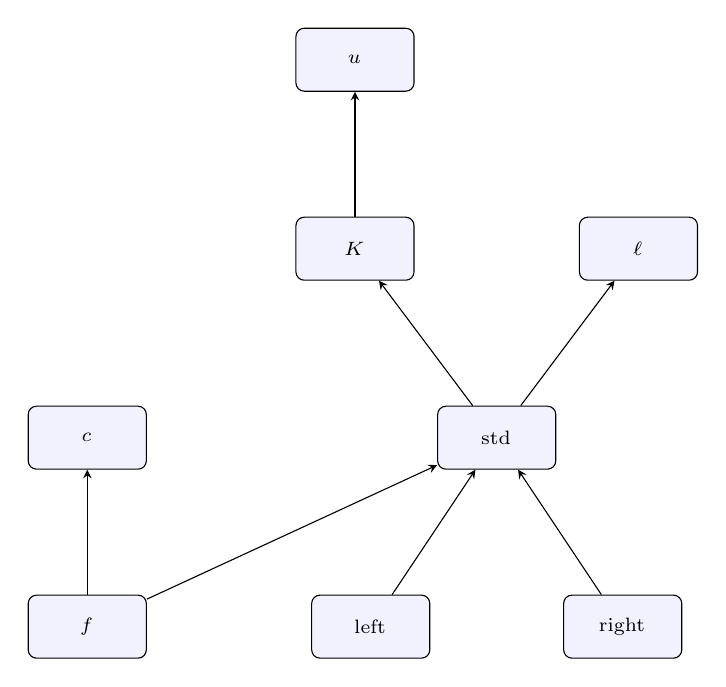
\begin{tikzpicture}[>=stealth,node distance=1cm,
  t/.style={draw,rounded corners=3pt,minimum width=1.5cm,minimum height=0.8cm,fill=blue!5}]
  \node[t] (f)  at (-5.2,0)   {$\T_f$};
  \node[t] (c)  at (-5.2,2.4) {$\T_c$};
  \node[t] (le) at (-1.6,0)   {$\T_{\mathrm{left}}$};
  \node[t] (ri) at (1.6,0)    {$\T_{\mathrm{right}}$};
  \node[t] (st) at (0,2.4)    {$\T_{\mathrm{std}}$};
  \node[t] (k)  at (-1.8,4.8) {$\T_K$};
  \node[t] (l)  at (1.8,4.8)  {$\T_\ell$};
  \node[t] (u)  at (-1.8,7.2) {$\T_u$};
  \draw[->] (f) -- (c);
  \draw[->] (f) -- (st);
  \draw[->] (le) -- (st);
  \draw[->] (ri) -- (st);
  \draw[->] (st) -- (k);
  \draw[->] (st) -- (l);
  \draw[->] (k) -- (u);
\end{tikzpicture}

\end{center}

\paragraph{Final summary.}
Strict chains: $\T_f\subsetneq\T_c$;
$\ \T_f,\T_{\mathrm{left}},\T_{\mathrm{right}}\subsetneq\T_{\mathrm{std}}$;
$\ \T_{\mathrm{std}}\subsetneq\T_K\subsetneq\T_u$; $\ \T_{\mathrm{std}}\subsetneq\T_\ell$.\\
Incomparable: $\T_K\parallel\T_\ell$, $\T_\ell\parallel\T_u$,
$\T_{\mathrm{left}}\parallel\T_{\mathrm{right}}$,
$\T_f\parallel\T_{\mathrm{left}},\T_{\mathrm{right}}$, and $\T_c$ is comparable only with $\T_f$
(where $\T_f\subsetneq\T_c$).
